\documentclass{article}

\usepackage{amsthm,amsmath,amssymb}
\usepackage[numbers]{natbib}
\usepackage{hyperref}
\usepackage{graphicx}
\usepackage{caption}
\usepackage{subcaption}
\newcommand{\bx}{{\mathbf x}}
\newcommand{\ba}{{\mathbf a}}
\newcommand{\bv}{{\mathbf v}}
\newcommand{\bu}{{\mathbf u}}

\usepackage{amsmath}
\DeclareMathOperator*{\argmax}{arg\,max}
\DeclareMathOperator*{\argmin}{arg\,min}


\newtheorem{theorem}{Theorem}[section]
\newtheorem{proposition}[theorem]{Proposition}
\newtheorem{lemma}[theorem]{Lemma}
\newtheorem{corollary}[theorem]{Corollary}
\newtheorem{remark}{Remark}[section]
\newtheorem{example}[theorem]{Example}


\begin{document}

\title{Management Sciences Topics: Convex Optimization\\ Midterm }
\date{}

\maketitle

\bigskip

\begin{enumerate}
\item Problem 1. 
\begin{enumerate}
\item 
$$
f(x, y) = \log(x^2+xy+y^2+1), \ x, y\in \mathbb{R}.
$$
Not convex. 

\item 
$$
f(x) = \exp(-\lVert Ax+b\rVert_2^2)
$$
Not convex.

\item
$$
f(x) = \exp(\lVert Ax+b\rVert_2^2)
$$
Convex. Let $f(x) = h\circ g(x)$, where $h(x) = \exp(x)$ is convex and increasing, and $g(x) = \lVert Ax+b\rVert_2^2 $ is convex. Hence $f$ is convex.

\end{enumerate}


\item Problem 2.

The Lagrange dual function is
$$
g(\lambda, \nu) = \inf_{x\in\mathbb{R}_+^n} \sum_{i=1}^{n}x_i\ln(x_i/y_i)+\sum_{i=1}^{n}\lambda_i(x_i-b_i)+\sum_{i=1}^{n}\lambda_i'(a_i-x_i) + \nu (\sum_{i=1}^{n}x_i-1),
$$
where $\lambda = (\lambda_i, \lambda_i') \in \mathbb{R}^{2n} $.
Then 
$$
\frac{\partial}{\partial x_i}g= \ln(x_i/y_i) + y_i + \lambda_i -\lambda_i' + \nu,
$$
so in order to get the minimum value for $g$, 
$$
x_i = y_i\exp(-y_i-\lambda_i+\lambda_i'-\nu).
$$
Then 
$$
\begin{aligned}
g(\lambda, \nu) &= \sum_{i=1}^{n}y_i(-y_i-\lambda_i+\lambda_i'-\nu)\exp(-y_i-\lambda_i+\lambda_i'-\nu) \\
&\quad + \sum_{i=1}^{n}\lambda_i(y_i\exp(-y_i-\lambda_i+\lambda_i'-\nu) - b_i) \\
&\quad + \sum_{i=1}^{n}\lambda_i'(a_i-y_i\exp(-y_i-\lambda_i+\lambda_i'-\nu)) \\
&\quad + \nu(\sum_{i=1}^{n}y_i\exp(-y_i-\lambda_i+\lambda_i'-\nu) - 1) \\
&= -\sum_{i=1}^{n}y_i^2 e^{-y_i-\lambda_i+\lambda_i'-\nu} - \sum_{i=1}^{n}\lambda_i b_i +\sum_{i=1}^{n} \lambda_i'a_i - \nu.
\end{aligned}
$$
Hence, the dual problem is
$$
\begin{aligned}
\text{maximize}&\quad -\sum_{i=1}^{n}y_i^2 e^{-y_i-\lambda_i+\lambda_i'-\nu} - \sum_{i=1}^{n}\lambda_i b_i +\sum_{i=1}^{n} \lambda_i'a_i - \nu \\
\text{subject to}&\quad \lambda_i \ge 0, \lambda_i' \ge 0.
\end{aligned}
$$

The KKT condition is
$$
\begin{aligned}
x_i-b_i\le 0,& \quad i = 1, \hdots, n \\
-x_i+a_i\le 0,& \quad i = 1, \hdots, n \\
\lambda_i \ge 0,& \quad i = 1, \hdots, n \\
\lambda_i' \ge 0,& \quad i = 1, \hdots, n \\
\lambda_i(x_i-b_i) = 0,& \quad i = 1, \hdots, n \\
\lambda_i'(-x_i+a_i) = 0,& \quad i = 1, \hdots, n \\
\ln(x_i/y_i)+y_i+\lambda_i-\lambda_i'+\nu_i = 0,& \quad i = 1, \hdots, n
\end{aligned}
$$
(I omitted the $*$ for each variable $x_i^*, \lambda_i^*, \lambda_i'^*, \nu_i^* $.)

\item Problem 3.

\begin{proof}
By definition, 
$$
\text{Prox}_h(z) = \argmin_{x\in \mathbb{R}^d} \frac{1}{2}\lVert x-z\rVert_2^2 + \lambda\lVert x\rVert_2. 
$$
Let
$$
f(x) = \frac{1}{2}\lVert x-z\rVert_2^2 + \lambda\lVert x\rVert_2,
$$
then by definition of subgradients,
$$
\partial f = \left\{
\begin{aligned}
x-z+\lambda\frac{x}{\lVert x\rVert_2},& \quad x \ne 0, \\
-z+\lambda\bar{B}(0, 1),& \quad x = 0,
\end{aligned}
\right.
$$
where $\bar{B}(0, 1)$ is the closed unit ball. Then 
\begin{enumerate}
\item If $\lVert z\rVert_2 > \lambda $, then $0\notin -z+\lambda\bar{B}(0, 1)$. In this case, the optimal $x $ satisfies $x\ne 0$ and
$$
x - z+\lambda\frac{x}{\lVert x\rVert_2} = 0.
$$
By solving this, we get
$$
x^* = (\lVert z\rVert_2 - \lambda)\frac{z}{\lVert z\rVert_2}.
$$
Since $x^*\ne 0 $, this holds when $\lVert z\rVert_2 > \lambda $.

\item When $\lVert z\rVert \le \lambda$, $0\in -z+\lambda\bar{B}(0, 1)$, while there's no such $x$ s.t. $x - z+\lambda\frac{x}{\lVert x\rVert_2} = 0$. Hence $x^* = 0$. Thus we have proved the statement.
\end{enumerate}
\end{proof}

\item Problem 4.

The code for this problem are \texttt{accelerated\_proximal\_gradient.m} and \texttt{elastic\_net\_regularized\_logistic\_regression.m}. The problem is formatted as 
$$
f(x) = g(x)+h(x), 
$$
where 
$$
g(x) = \frac{1}{n}\sum_{i=1}^{n}\log(1+\exp(-b_ia_i^\top x) +\frac{\lambda_2}{2}\lVert x\rVert_2^2,
$$
and 
$h(x) = \lambda_1\lVert x\rVert_1 $, so as to guarantee the strongly convexity of $g$. 

However, if I choose $x_0  = 0$, I have $x_1 = x_0 $ exactly, so the iteration cannot continue, which does not agree with the properties. 

\item Problem 5.

The code for this problem are \texttt{stochastic\_subgradient.m} and \texttt{sparse\_hinge\_loss.m}.
\begin{figure}
\centering
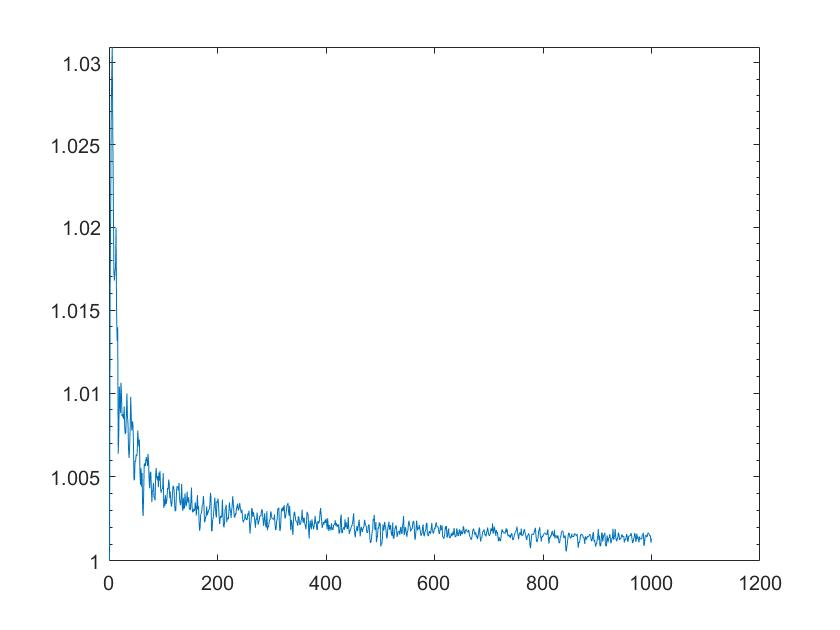
\includegraphics[scale=0.4]{problem5.jpg}
\caption{Convergence plot for SSG}
\label{problem 5}
\end{figure}


\end{enumerate}

\end{document}

